\documentclass[a4paper,14pt]{extarticle}

\usepackage[T2A]{fontenc}			
\usepackage[utf8]{inputenc}			
\usepackage[english,russian]{babel}

\usepackage[
bookmarks=true, colorlinks=true, unicode=true,
urlcolor=black,linkcolor=black, anchorcolor=black,
citecolor=black, menucolor=black, filecolor=black,
]{hyperref}

\usepackage{color}
\usepackage{caption}
\DeclareCaptionFont{white}{\color{black}}
\DeclareCaptionFormat{listing}{\colorbox{white}{\parbox{\textwidth}{#1#2#3}}}
\captionsetup[lstlisting]{format=listing,labelfont=white,textfont=white}

\usepackage{amsmath,amsfonts,amssymb,amsthm,mathtools} 
\usepackage{wasysym}

\usepackage{graphicx}
%\usepackage[cache=false]{minted}
\usepackage{cmap}
\usepackage{indentfirst}

\usepackage{listings} 
\usepackage{fancyvrb}

\usepackage{geometry}
\geometry{left=2cm}
\geometry{right=1.5cm}
\geometry{top=1cm}
\geometry{bottom=2cm}

\setlength{\parindent}{5ex}
\setlength{\parskip}{0.5em}

\usepackage{color}
\usepackage[cache=false, newfloat]{minted}
\newenvironment{code}{\captionsetup{type=listing}}{}
\SetupFloatingEnvironment{listing}{name=Листинг}
 
 
 \begin{document}
 	
 	\def\figurename{Рисунок}
 	
 	\begin{minipage}{0.2\textwidth}
 		
\includegraphics[scale=0.05]{img/bmstu.png}
 	\end{minipage}
 	\begin{minipage}{0.7\textwidth}
 		\small
 		\begin{center}
 			\textbf{Министерство науки и высшего образования Российской Федерации}
 			
 			\textbf{Федеральное государственное бюджетное образовательное учреждение высшего образования «Московский государственный технический университет имени Н.Э. Баумана}
 			
 			\textbf{(национальный исследовательский университет)»}
 			
 			\textbf{(МГТУ им. Н.Э. Баумана)}
 		\end{center}
 	\end{minipage}
 	
 	\vspace*{5mm}
 	
 	\vspace*{30mm}
 	
 	\LARGE
 	\begin{center}
 		\textbf{Рубежный контроль №2}
 		
 		%	\textbf{к курсовому проекту на тему:}
 		\textbf{Реферат на тему:}
 		
 		\textbf{<<Хозяйственные средства и их содержание. Основные и оборотные средства
 			предприятия – внеоборотные и оборотные активы.>>}
 	\end{center}
 	
 	%\huge
 	%\begin{center}
 	%	\textbf{Лабораторная работа №9}
 	%\end{center}
 	%
 	%\begin{center}
 	%	\textbf{Тема:} <<Обработчики прерываний>>
 	%\end{center}
 	
 	\vspace*{15mm}
 	
 	\large
 	\begin{flushleft}
 		\textbf{Дисциплина:} Экономика \\
 		\textbf{Студент:} Левушкин И. К. \\
 		\textbf{Группа:} ИУ7-72Б \\
 		%        \textbf{Оценка (баллы):} \\
 		\textbf{Преподаватель:} Герцик Ю.Г.\\
 	\end{flushleft}
 	
 	\vspace*{50mm}
 	
 	\large
 	\begin{center}
 		Москва, 2020 г.
 	\end{center}
 	
 	\thispagestyle{empty}
 	
 	\newpage
 	
 	\tableofcontents
 	\newpage
 	\section*{Введение}
 	\addcontentsline{toc}{section}{Введение}
 	
 	Хозяйственные средства организации – товарно-материальные ценности и денежные средства, как принадлежащие организации, так и временно или постоянно находящиеся вне ее собственности. Они являются активом организации и классифицируются по составу: внеоборотные и оборотные средства.
 	
 	Целью работы является рассмотрение сложившейся структуры
 	хозяйственных средств организации.
 	
 	\newpage
 	
 	\section{Классификация хозяйственных средств}
 	
 	Состав хозяйственных средств достаточно разнообразен. Он определяется содержанием, отраслевыми особенностями, объектом хозяйственной деятельности предприятия.
 	
 	Хозяйственные средства (имущество) любого предприятия в целях их правильного отражения в бухгалтерском учете группируются по двум признакам: по их функциональной роли в процессе производства и по источникам их формирования (рис. \ref{ris:1}).
 	
 	\begin{figure}[h!]
 		\begin{center}
 			{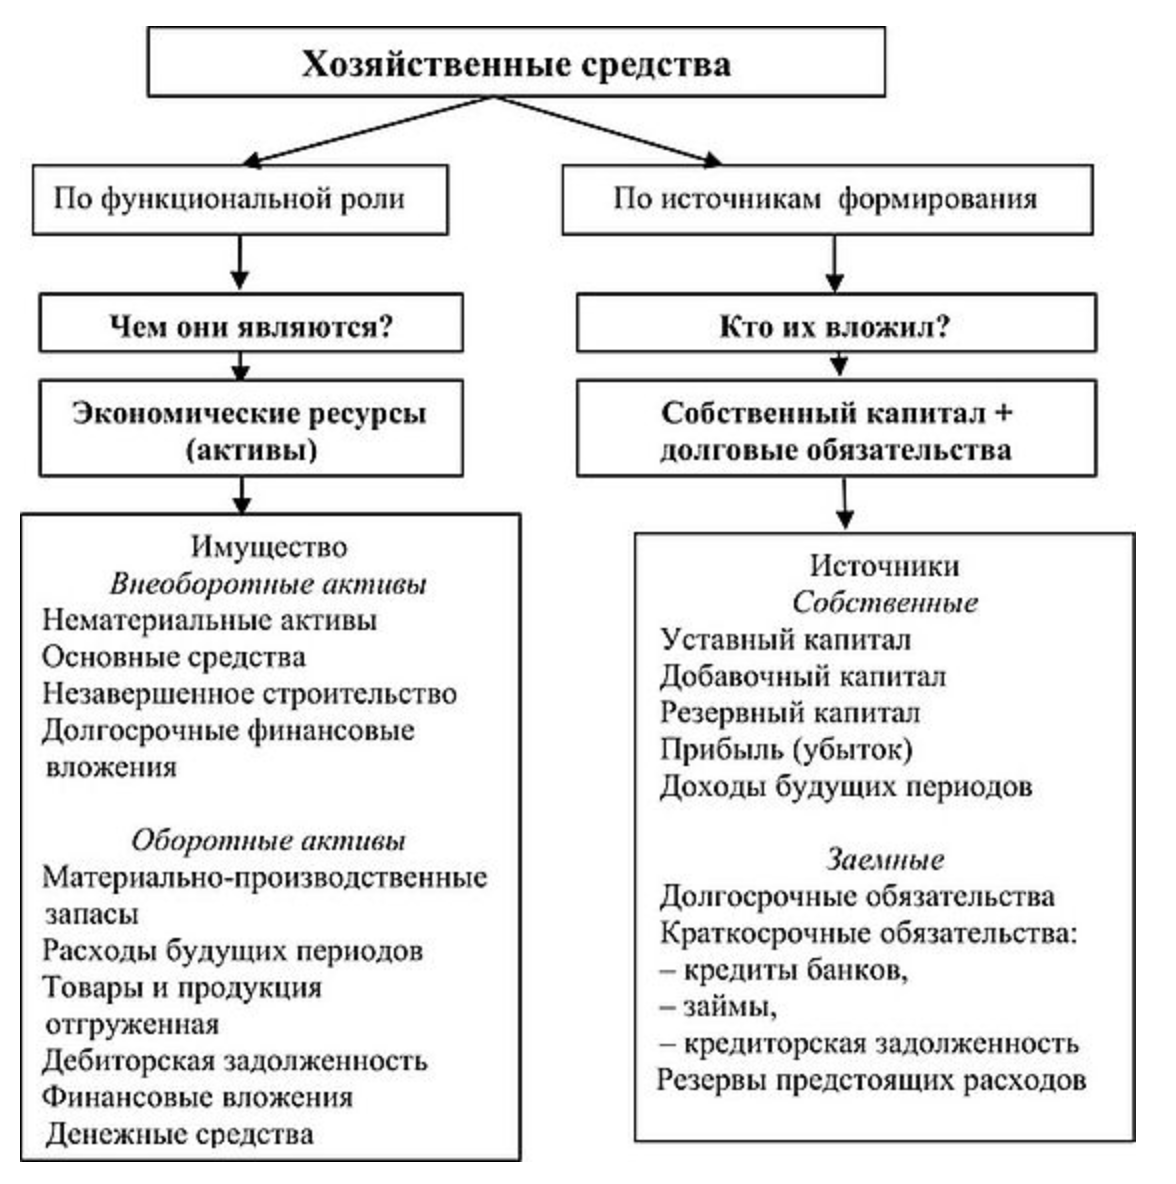
\includegraphics[scale = 0.4]{1.png}}
 		\end{center}
 		\caption{Классификация хозяйственных средств по функциональной роли в процессе производства и по источнкам их формирования}
 		\label{ris:1}
 	\end{figure}
 
 В зависимости от функциональной роли в процессе производства хозяйственные средства представлены экономическими ресурсами, классифицированными по сроку их участия в производственном процессе. Если экономические ресурсы используются в производственном процессе более года, они являются долгосрочными (внеоборотными) активами, если менее года, то текущими (оборотными) активами.
 
 \section{Внеоборотные активы}
 
 Внеоборотные активы являются средствами длительного пользования, они функционируют в течение нескольких отчетных периодов. К ним относятся (рис. \ref{ris:1}):
 
 \subsection{Нематериальные активы}
 
 Нематериальные активы (НМА) — это средства, не имеющие видимой материальной формы, но способные приносить их владельцу непосредственный доход и обеспечивать необходимые условия его извлечения.
 
 К нематериальным активам, используемым в течение длительного периода (свыше одного года) в хозяйственном кругообороте капитала, относят:
 
 \begin{itemize}
 	\item права, возникающие из авторских и иных договоров на произведения науки, литературы, искусства и объекты смежных прав, на программы ЭВМ, базы данных и др.;
 	\item права, возникающие из патентов на изобретения, промышленные образцы, селекционные достижения, из свидетельств на полезные модели, товарные знаки, торговые марки, «ноу-хау»;
 	\item права пользования земельными участками, природными ресурсами и организационные расходы при создании предприятия.
 \end{itemize}
 
 \subsection{Основные средства}
 
 Основные средства — это часть имущества, используемая в качестве средств труда при производстве продукции, выполнении работ или оказании услуг либо для управления организацией в течение периода, превышающего 12 месяцев или обычный операционный цикл, если он превышает 12 месяцев. Согласно Положению по ведению бухгалтерского учета и отчетности в России к основным средствам относятся: предметы, служащие более года независимо от их стоимости.
 
 К основным средствам относятся: 
 \begin{itemize}
 	\item здания;
 	\item сооружения;
 	\item оборудование;
 	\item вычислительная техника;
 	\item транспортные средства;
 	\item хозяйственный инвентарь;
 	\item инструменты;
 	\item и так далее.
 \end{itemize}

Особенность основных средств состоит в том, что они многократно участвуют в процессе производства продукции и в течение периода эксплуатации на объекты основных средств начисляется \textit{амортизация}.

{\bf Амортизация} — это постепенное включение стоимости объектов основных средств в себестоимость выпускаемой продукции (работ, услуг) в течение нормативного срока их использования.

\newpage
 
 \section{Оборотные активы}
 
 Оборотные активы отличаются от средств длительного пользования (основных средств, нематериальных активов) тем, что они могут быть обращены в деньги или полностью использованы в ближайшем будущем (в течение одного года или операционного цикла). Они участвуют в одном кругообороте капитала, их стоимость сразу переносится на готовый продукт и полностью списывается на затраты предприятия.
 
 Краткосрочные (оборотные, текущие) активы подразделяются на \textit{денежные} и \textit{неденежные} активы.
 
 Оборотные активы с точки зрения экономической теории делятся на 
 \begin{itemize}
 	\item предметы труда;
 	\item продукты труда;
 	\item денежные средства;
 	\item средства в расчетах;
 	\item финансовые вложения.
 \end{itemize}

\newpage

\subsection{Оборот текущих (оборотных) активов}

{\bf Предметы труда} — часть средств производства, на которую воздействует человек в процессе труда при помощи средств труда. Предметы труда однократно участвуют в процессе производства и целиком переносят свою стоимость на изготавливаемую продукцию. 

К ним относятся: 
\begin{itemize}
	\item сырье;
	\item материалы;
	\item топливо;
	\item полуфабрикаты;
	\item незавершенное производство;
	\item запасные части;
	\item тара.
\end{itemize}

Под \textit{сырьем} понимают продукцию сельского хозяйства и добывающих отраслей промышленности, а под \textit{материалами} — продукцию обрабатывающих отраслей.

Материалы по их роли в процессе изготовления продукции делятся на две группы: сырье и основные материалы (составляют вещественную основу продукта); вспомогательные материалы используются для выполнения определенных функций.

\textit{Топливо} по своей роли в процессе производства относится к вспомогательным материалам, но, поскольку оно занимает большой удельный вес в себестоимости продукции и выполняет особые функции в процессе производства, в бухгалтерском учете его выделяют в отдельную группу.

\textit{Полуфабрикаты} — предметы труда, которые прошли обработку в одном или нескольких подразделениях организации, но подлежат дальнейшей обработке в данной организации или вне ее.

К \textit{незавершенному производству} относят предметы труда, находящиеся на обработке в подразделениях на рабочих местах.

К {\bf продуктам труда} относятся 
\begin{itemize}
	\item выпуск продукции (работ, услуг);
	
	\item товары – товарно-материальные ценности, приоб­ретенные в качестве товаров для продажи;
	
	\item торговая наценка;
	
	\item готовая продукция на складе организации, предназначенная для реализации;
	
	\item расходы на продажу, связанные с продажей про­дукции, товаров, работ и услуг;
	
	\item товары отгруженные – отгруженная продукция, выручка от продажи которой определенное время не может быть признана в бухгалтерском учете, а также готовые изделия, переданные другим организациям для продажи на комиссионных началах;
	
	выполненные этапы по незавершенным работам.
\end{itemize}

Под {\bf средствами в расчетах} понимают долги юридических или физических лиц данной организации. Такая задолженность называется дебиторской, а сами должники — дебиторами. Дебиторская задолженность возникает в результате действующих форм расчетов за продукцию, работы и услуги в том случае, если их передача покупателю и платежи за них не совпадают во времени. Дебиторами могут быть и работники организации. Таких должников называют подотчетными лицами.

{\bf Денежные средства} – денежная наличность в российской и иностранных валютах, находящаяся в кассе, на расчетных, валютных и других счетах, открытых в кре­дитных организациях на территории страны и за ее пре­делами, а также ценные бумаги, платежные и денежные документы:
\begin{itemize}
	\item касса;
	\item расчетные счета – денежные средства в валюте РФ на расчетных счетах организации, открытых в кре­дитных организациях;
	\item валютные счета – денежные средства в иностран­ной валюте на валютных счетах организации, открытых в кредитных организациях на территории Российской Федерации и за ее пределами;
	\item специальные счета в банках – денежные средства в валюте РФ и иностранных валютах, находящиеся на территории Российской Федерации и за ее пре­делами в аккредитивах, чековых книжках, иных платежных документах, на текущих, особых и иных специальных счетах;
	\item переводы в пути – денежные суммы, внесенные в кассы кредитных организаций, кассы почтовых от­делений для зачисления на расчетный или иной счет организации, но еще не зачисленные по назначе­нию;
	\item {\bf финансовые вложения} – инвестиции организации в государственные ценные бумаги, акции, облига­ции, а также предоставленные другим организаци­ям займы;
	
	\item расчеты с покупателями и заказчиками;
	
	\item расчеты с подотчетными лицами (расчеты с работ­никами по суммам, выданным им под отчет на ад­министративно-хозяйственные и операционные рас­ходы);
	
	\item расчеты с разными дебиторами.
\end{itemize}

Дебиторская задолженность – это задолженность различных организаций или отдельных лиц данной орга­низации.

Дебиторами называются организации или отдельные лица, которые используют средства данной организации.

Расходы будущих периодов представляют собой определенные текущие активы неосязаемого характера, полезность которых закончится в обозримом будущем (отдельные затраты, связанные с освоением производства и подготовкой кадров).
 	
 	\newpage
 	\section{Заключение}
 	\addcontentsline{toc}{section}{Заключение}
 	
 	В данной работе приведено определение хозяйственных средств организаций. Была дана классификация хозяйственных средств по их функциональной роли в процессе производства и по источникам их формирования.
 	
 	Было изучена структура внеоборотных и оборотных активов, а также даны определения ключевых понятий данных областей.
 	
 	В итоге, поставленная цель, заключающаяся в исследовании
 	структуры хозяйственных средств, достигнута.
 	
 	\newpage
 	
 	
 	\addcontentsline{toc}{section}{Список используемой литературы}
 	\begin{thebibliography}{3}
 		\bibitem{first}
 		Классификация хозяйственных средств [Электронный ресурс]. – Режим доступа: 
 		https://studref.com/313367/buhgalterskiy\_uchet\_i\_audit/klassifikatsiya\_hozyaystvennyh\_sredstv, 
 		свободный – (02.11.2020)
 		\bibitem{second} Классификация хозяйственных средств предприятия [Электронный ресурс]. – Режим доступа: 
 		https://infopedia.su/2x71b5.html, 
 		свободный – (02.11.2020)
 		\bibitem{third} Бухгалтерский учет П. В. Николаев [Электронный ресурс]. – Режим доступа: 
 		http://library.miit.ru/methodics/04022015/03-42902.pdf, 
 		свободный – (02.11.2020)
 	\end{thebibliography}
 	
 \end{document}